\cleardoublepage
\newpage
\section*{DISCUSIÓN}
\addcontentsline{toc}{section}{DISCUSIÓN}
\par\refstepcounter{section}
\subsection{Pruebas en proteínas}
\par
La primera prueba que se le hace a los nuevos potenciales BSASA y SASA es la clasificación de estructuras en nativas y no nativas, un problema considerado ya resuelto por una gran cantidad de software y métodos publicados. (citar metodos)
En la figura~\ref{fig:ferrada2009} podemos observar como los potenciales de la metodología nueva utilizando subsuperfices y la combinación con potenciales de superfície tienen peores resultados que los que utilizan distancias y la combinación de conteo de átomos y distancia.
Esto se debe al rango de interacción más corto que tienen los potenciales BSASA, que impide el reconocomiento de posibles interacciones no favorables más distantes (figura~\ref{fig:radii_int}) que no es capaz de observar ya que el rango máximo de distancia es equivalente a dos veces el radio de Van der Waals más 1.4 \si{\angstrom} de distancia, siendo 1.4 \si{\angstrom} el radio de una molécula de agua.
En la figura~\ref{fig:radii_int} podemos ver las distribuciones de la cantidad de interacciones entre pares de átomos para las estructuras utilizadas en la derivación de los potenciales en proteína.
\begin{figure}[!p]
\centering
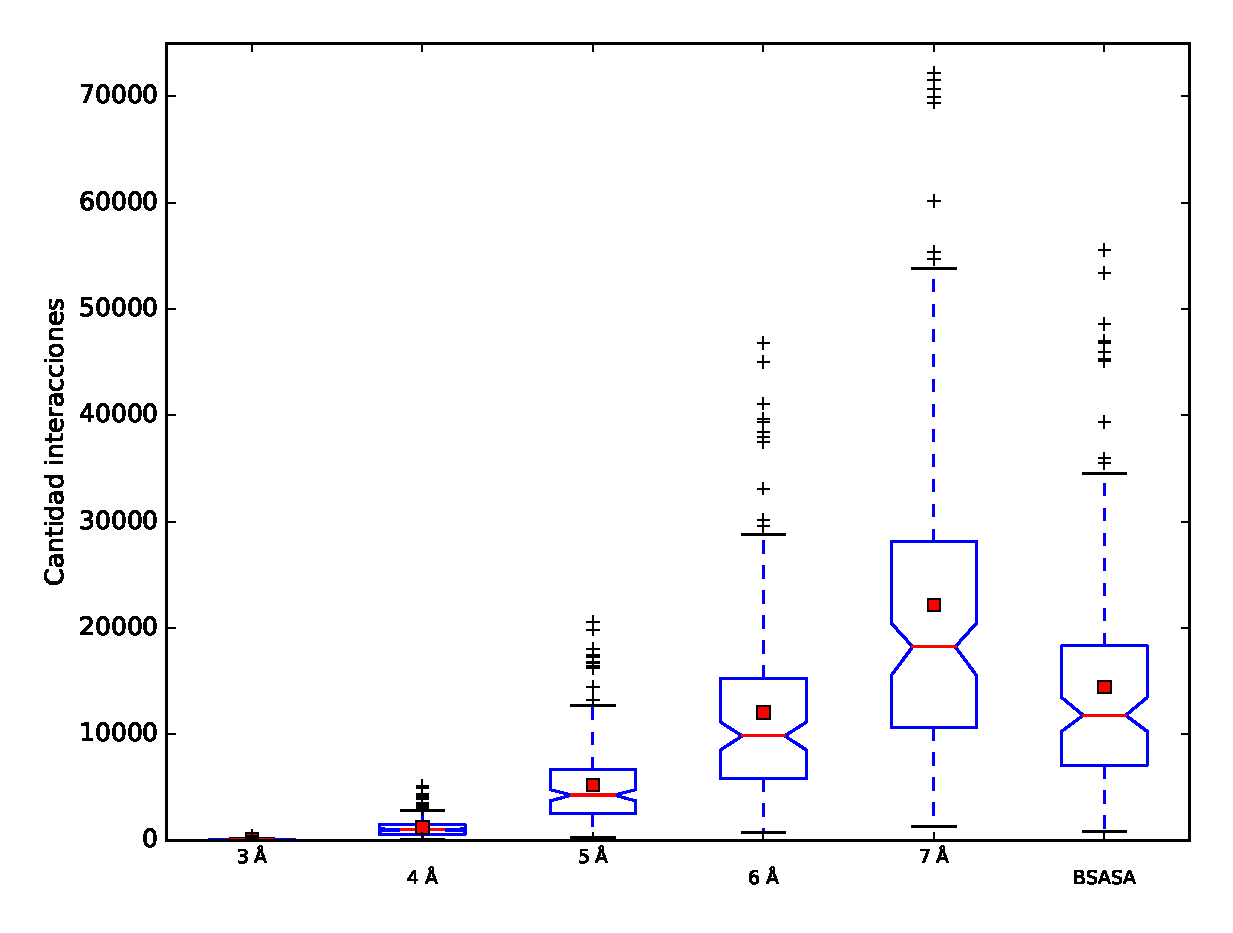
\includegraphics[width=\linewidth]{figures/radii_int.eps}
\caption[Boxplots de las distribuciones de la cantidad de contactos encontrados en el conjunto de estructuras usado en la derivación de potenciales para proteínas.]{Boxplots de las distribuciones de la cantidad de contactos encontrados en el conjunto de estructuras usado en la derivación de potenciales para proteínas. En la figura se tienen las distribuciones de la cantidad de contactos para potenciales dependientes de distancia variando el radio máximo de interacción de 3 a 7 \si{\angstrom}, más el potencial BSASA. La línea roja indica la mediana, el punto rojo el promedio, y la cintura el intervalo de confianza.}
\label{fig:radii_int}
\end{figure}
La distribución para BSASA muestra que el potencial evalua una menor cantidad de interacciones que los potenciales de distancia, que usan un rango de máximo de 7 \si{\angstrom} para evaluar interacciones.
De acuerdo a la ecuación~\ref{ec:ip} esto implica directamente que el potencial BSASA tiene un menor contenido de información disponible para la evaluación de la estructura, dado el menor número de interacciones pareadas observadas, que es el término \textit{n} en la ecuación.
Entre tanto, el potencial SASA logra un mucho mejor desempeño que conteo, dado que es mucho más fino en registrar si un átomo esta enterrado o expuesto, ya que se mide directamente la superficie en contacto con el solvente, en vez del método indirecto del potencial de conteo.
\par
En la segunda prueba, la capacidad de los nuevos potenciales BSASA y SASA en detectar errores aislados y expuestos en la superficie, tanto como errores más internos y difíciles de detectar fue evaluada utilizando perfiles de energía, en vez de usar el valor promedio de energía como en las pruebas anteriores.
Estos perfiles de energía contienen valores de energía promediados en una ventana deslizante de 7 residuos lo que permite eliminar variaciones bruscas en los valores de energía de cada residuo.
En esta prueba el valor final de energía de cada residuo se evalúa como un elemento independiente.
Al evaluar los errores de clase A, notamos que el desempeño de los pares de potenciales comparables no es distinguible, excepto en el caso de los potenciales SASA y CONTEO.
Dado que los errores en los residuos clase A son en residuos aislados y expuestos, el mejor desempeño de SASA versus CONTEO era esperado.
A su vez, los potenciales DD y BSASA y sus respectivas combinaciones DD+CONTEO y BSASA+SASA no muestran diferencias significativas en estos modelos.
Pero en los modelos clase B, cuyos residuos poseen errores más internos en la estructura afectando también residuos correctamente modelados su alrededor o entorno local, los potenciales BSASA y BSASA+SASA logran un desempeño superior a los potenciales DD y DD+CONTEO.
Esto se debe a la capacidad del potencial BSASA de excluir naturalmente los contactos que están escondidos detrás de otros átomos, algo que los potenciales de distancia no pueden detectar normalmente sin utilizar algoritmos para la detección de esos casos. (\cite{Ferrada2007,Ferrada2009})

\subsection{Pruebas en ARN}
En la primera prueba se observó la correlación del valor de energía calculado por los potenciales con las medidas de desviación estructural de más de 80 estructuras con 500 modelos cada una.
Esta prueba es muy similar a la primera prueba en proteínas, que buscaba separar modelos entre nativos y no nativos, que no es aún posible realizar dada la falta de una base de datos de estructuras y modelos de ARN ya clasificados en nativos y no nativos.
Al igual que en la primera prueba en proteínas, los potenciales BSASA y su combinación BSASA+SASA tienen un desempeño menor al potenciales de referencia RASP.
El potencial RASP utiliza un rango de 20 \si{\angstrom} para la detección de interacciones, lo que significa que es capaz de detectar y evaluar motifs de estructuras terciarias estadísticamente probables de estar en proximidad.
En la figura~\ref{fig:radii_rna} apreciamos como el potencial RASP mide casi una unidad de magnitud más contactos que el potencial BSASA.
\begin{figure}[!p]
\centering
\includegraphics[width=\linewidth]{figures/radii_rna.eps}
\caption[Boxplots de las distribuciones de la cantidad de contactos encontrados en el conjunto de estructuras usado en la derivación de potenciales para ARN.]{Boxplots de las distribuciones de la cantidad de contactos encontrados en el conjunto de estructuras usado en la derivación de potenciales para ARN. En la figura se tienen las distribuciones de la cantidad de contactos para potenciales dependientes de distancia variando el radio máximo de interacción de 5 a 20 \si{\angstrom}, más el potencial BSASA. La línea roja indica la mediana, el punto rojo el promedio, y la cintura el intervalo de confianza.}
\label{fig:radii_rna}
\end{figure}
\par
Pero en la segunda prueba, la cual se realiza utilizando fragmentos de RNA de menor tamaño, podemos apreciar como el potencial BSASA tiene mejor desempeño que RASP.
Dado que se usan fragmentos pequeños de ARN, ocurre un efecto similar a lo que ocurre en la utilización de residuos en vez de la estructura completa, como en el segundo experimento en proteínas.
Estos resultados indican que el potencial BSASA tiene una mejor desempeño al evaluar estructuras pequeñas (fragmentos) o errores locales en estructuras completas.

\subsection{Pruebas en ADN}
La prueba realizada en se enfoca en la capacidad del potencial en identificar el modelo más cercano a uno nativo. Esta prueba se asemeja al primer experimento realizado en ARN.
En este caso se utilizan los modelos ya generados por el método con restricciones adicionales a MODELLER creado por \cite{Ilibarra2013}, en los cuales se generan modelos utilizando para una determinada secuencia de ADN derivando parámetros a partir de otras estructuras, excluyendo la estructura con la secuencia pedida del conjunto de datos.
El potencial utilizado en este caso también posee las mismas restricciones, por lo que la estructura original no está en su conjunto de entrenamiento, lo que nos permite eliminar sesgos en la evaluación de los modelos.
En la primera prueba, en donde se utilizan las restricciones de modelaje generadas a partir del set no redundante de estructuras de ADN, no se observaron diferencias significativas en el desempeño de los potenciales para encontrar los mejores modelos. 
Entretanto, para los modelos generados utilizando los parámetros por defecto del software MODELLER, solo se encontraron diferencias significativas entre los potenciales DD, DD+SASA y SASA.
Al analizar algunas de las estructuras encontradas y los datos de la figura~\ref{fig:dna1}, podemos ver como los potenciales fallan en encontrar los modelos de menor RMSD, en algunos casos encontrando modelos con diferencias mínimas, como en la figura~\ref{fig:dnatest1} y en otros seleccionando modelos con más de 4 \si{\angstrom} comparados con el modelo de menor RMSD encontrado como en la figura~\ref{fig:dnatest2}.

\begin{figure}[!p]

  \begin{subfigure}{.5\linewidth}
    \includegraphics[width=\linewidth]{figures/discusion/rsron/1d65_best.png}
    \caption{}
  \end{subfigure}%
~
  \begin{subfigure}{.5\linewidth}
    \includegraphics[width=\linewidth]{figures/discusion/rsron/1d65_rmsd.png}
    \caption{}
  \end{subfigure}

  \begin{subfigure}{.5\linewidth}
    \includegraphics[width=\linewidth]{figures/discusion/rsron/181d_best.png}
    \caption{}
  \end{subfigure}%
~
   \begin{subfigure}{.5\linewidth}
    \includegraphics[width=\linewidth]{figures/discusion/rsron/181d_rmsd.png}
    \caption{}
  \end{subfigure}


\caption[Superposiciones con el cristal original de algunos de los mejores modelos de ADN encontrados según los potenciales, para el conjunto generado con restricciones.]{Superposiciones de algunos modelos generados para una secuencia especifica con su cristal original para el conjunto sin restricciones de modelamiento. En todas las figuras los modelos de color rojo son el cristal original, mientras que superpuesto en azul está el modelo generado. En (a) se tiene el mejor modelo para la secuencia de la estructura 1D65 encontrado por el potencial BSASA, y en (b) el modelo con el menor RMSD, que en este caso fueron el mismo. En (c) y (d) se tiene uno de los peores resultados, con (c) mostrando el mejor modelo encontrado para el potencial BSASA para la estructura 181D con un dRMSD de 6.582 \si{\angstrom} contra el modelo de menor RMSD encontrado en (d).}
\label{fig:dnatest1}
\end{figure}

\begin{figure}[!p]

  \begin{subfigure}{.5\linewidth}
    \includegraphics[width=\linewidth]{figures/discusion/rsroff/424d_best.png}
    \caption{}
  \end{subfigure}%
~
  \begin{subfigure}{.5\linewidth}
    \includegraphics[width=\linewidth]{figures/discusion/rsroff/424d_rmsd.png}
    \caption{}
  \end{subfigure}

  \begin{subfigure}{.5\linewidth}
    \includegraphics[width=\linewidth]{figures/discusion/rsroff/3ew9_best.png}
    \caption{}
  \end{subfigure}%
~
   \begin{subfigure}{.5\linewidth}
    \includegraphics[width=\linewidth]{figures/discusion/rsroff/3ew9_rmsd.png}
    \caption{}
  \end{subfigure}

\caption[Superposiciones con el cristal original de algunos de los mejores modelos de ADN encontrados según los potenciales, para el conjunto generado sin restricciones]{Superposiciones de algunos modelos generados para una secuencia especifica con su cristal original para el conjunto sin restricciones de modelamiento. En todas las figuras los modelos de color rojo son el cristal original, mientras que superpuesto en azul está el modelo generado. En (a) se tiene el mejor modelo para la secuencia de la estructura 424D encontrado por el potencial BSASA, y en (b) el modelo con menor RMSD. En (c) tenemos el caso de 3EW9, donde el potencial BSASA no logra encontrar el mejor modelo, y en (d) tenemos el modelo de menor RMSD con el cristal.}
\label{fig:dnatest2}
\end{figure}

Esto indica que los parámetros utilizados para los potenciales en ARN no son los óptimos para estructuras de ADN, o que el conjunto de entrenamiento utilizado no posee las características necesarias para generar potenciales capaces de una mejor discriminación entre los modelos específicos utilizados en esta prueba.

Otro efecto observado fue que la combinación DD+SASA entregó resultados casi idénticos en ambas pruebas, lo que indica que la fórmula utilizada para ajustar la proporción del valor de energía que entrega cada potencial puede no ser óptima al evaluar estructuras de ADN. 
